% Part V — Causal Study  |  ~10 slides  |  Madrid/seahorse  |  16:9
\documentclass[aspectratio=169,10pt]{beamer}
\usetheme{Madrid}\usecolortheme{seahorse}
\usepackage{tikz}
\usetikzlibrary{arrows.meta,shapes,positioning}
\usepackage{pgfplots}\pgfplotsset{compat=1.17}
\usepackage{booktabs,amsmath,amssymb,xcolor}
\definecolor{myblue}{RGB}{0,50,130}
\definecolor{myred}{RGB}{153,0,0}
\definecolor{mygreen}{RGB}{0,100,50}
\definecolor{myorange}{RGB}{180,80,0}
\newcommand{\NHOP}{\mathrm{NHOP}}
\newcommand{\IR}{\mathrm{IR}}
\setbeamertemplate{navigation symbols}{}
\title[Part V: Causal Study]{Part V — Causal Study}
\subtitle{Does Class Imbalance \emph{Cause} Classifier Degradation?}
\author{Parsa Hajiannejad}\date{2026}

\begin{document}
\begin{frame}\titlepage\end{frame}

% ----- Slide 1 ---------------------------------------------------------------
\begin{frame}{The Untested Assumption}
\begin{columns}[T]
\column{0.50\textwidth}
\textbf{Every oversampling paper assumes} imbalance degrades classifiers.\\[6pt]
But prior work confounds three effects:
\begin{itemize}
  \item \textbf{Distributional shift}: removing instances changes minority shape
  \item \textbf{Sample size reduction}: fewer minority instances = less information
  \item \textbf{Imbalance ratio per se}: the ratio itself biases decision boundaries
\end{itemize}
\vspace{6pt}
\textbf{Our design:} use NHOP-guided greedy removal to increase IR \emph{while preserving the minority distributional shape}. Any performance drop is then causally attributable to IR alone.

\column{0.48\textwidth}
\begin{center}
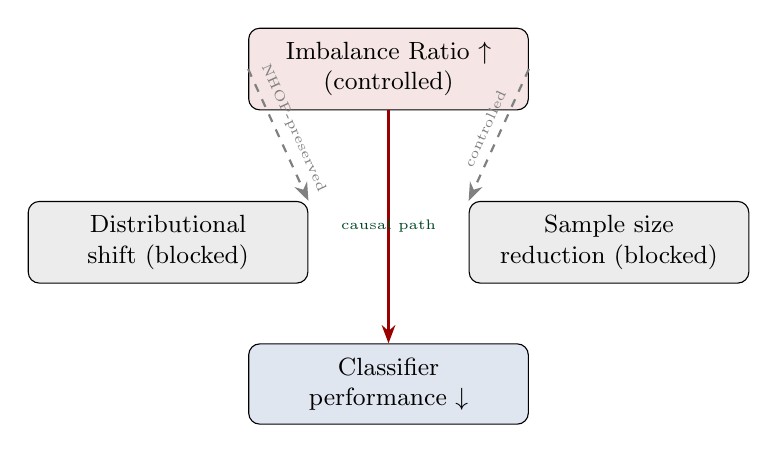
\begin{tikzpicture}[
  node/.style={rectangle,rounded corners=4pt,draw,text width=3.2cm,
               align=center,font=\small,inner sep=5pt}]
\node[node,fill=myred!10]   (ir)   at (0,2.2)  {Imbalance Ratio $\uparrow$\\(controlled)};
\node[node,fill=gray!15]    (ds)   at (-2.8,0) {Distributional\\shift (blocked)};
\node[node,fill=gray!15]    (ss)   at (2.8,0)  {Sample size\\reduction (blocked)};
\node[node,fill=myblue!12]  (perf) at (0,-1.8) {Classifier\\performance $\downarrow$};
\draw[-{Stealth},myred,thick] (ir.south) -- (perf.north);
\draw[-{Stealth},gray,dashed,thick] (ir.west) -- node[above,font=\tiny,sloped]{NHOP-preserved} (ds.north east);
\draw[-{Stealth},gray,dashed,thick] (ir.east) -- node[above,font=\tiny,sloped]{controlled} (ss.north west);
\node[font=\tiny,mygreen!70!black] at (0,0.2) {causal path};
\end{tikzpicture}
\end{center}
\end{columns}
\end{frame}

% ----- Slide 2 ---------------------------------------------------------------
\begin{frame}{Protocol: Degradation then Recovery}
\begin{columns}[T]
\column{0.50\textwidth}
\textbf{Phase 1 — Degradation:}\\
Greedy removal of minority instances one at a time, selecting at each step the instance whose removal \emph{minimises NHOP reduction}:
\[
  x^* = \arg\min_{x \in \mathcal{M}} \Delta\NHOP(x)
\]
Sweep from balanced ($\IR=1$) to 70\% removed ($\IR\approx4$).

\vspace{8pt}
\textbf{Phase 2 — Recovery:}\\
Apply 7 oversamplers incrementally from the most-degraded state back to balance. Evaluated on 5 classifiers, 6 metrics, 10 datasets.

\vspace{6pt}
\textbf{LeakageSafeCV} (4-rule protocol) prevents 2--5\% AUC inflation from oversampling leakage — prevents false method rankings.

\column{0.48\textwidth}
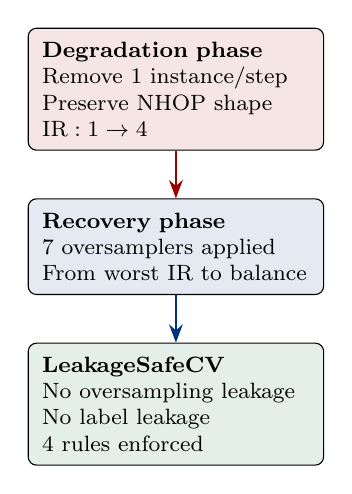
\begin{tikzpicture}[
  pnode/.style={rectangle,rounded corners=3pt,draw,text width=3.4cm,
               align=left,font=\footnotesize,inner sep=5pt}]
\node[pnode,fill=myred!10]    (d1) at (0,0)   {\textbf{Degradation phase}\\Remove 1 instance/step\\Preserve NHOP shape\\$\IR: 1 \to 4$};
\node[pnode,fill=myblue!10]   (d2) at (0,-2.0) {\textbf{Recovery phase}\\7 oversamplers applied\\From worst IR to balance};
\node[pnode,fill=mygreen!10]  (d3) at (0,-4.0) {\textbf{LeakageSafeCV}\\No oversampling leakage\\No label leakage\\4 rules enforced};
\draw[-{Stealth},myred,thick]  (d1.south)--(d2.north);
\draw[-{Stealth},myblue,thick] (d2.south)--(d3.north);
\end{tikzpicture}
\end{columns}
\end{frame}

% ----- Slide 3 ---------------------------------------------------------------
\begin{frame}{Degradation: Performance Collapses at IR $\approx$ 2}
\begin{columns}[T]
\column{0.54\textwidth}
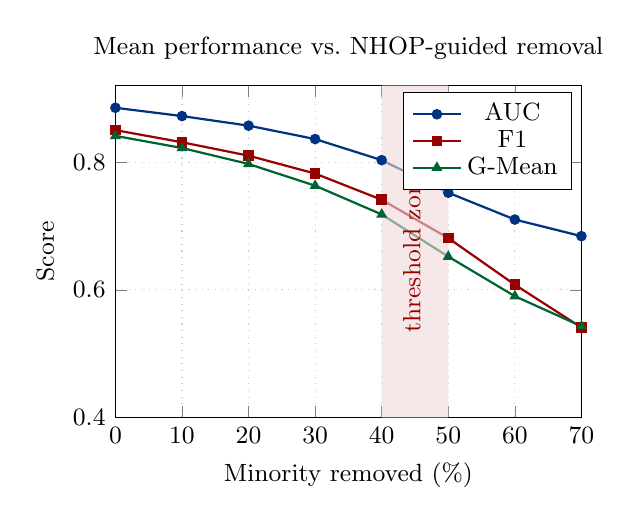
\begin{tikzpicture}
\begin{axis}[
  width=7.5cm,height=5.8cm,
  xlabel={\small Minority removed (\%)},
  ylabel={\small Score},
  xmin=0,xmax=70,ymin=0.40,ymax=0.92,
  xtick={0,10,20,30,40,50,60,70},
  xticklabel style={font=\small},
  yticklabel style={font=\small},
  xlabel style={font=\small},
  ylabel style={font=\small},
  title={\small Mean performance vs.\ NHOP-guided removal},
  title style={font=\small},
  legend style={font=\small,at={(0.98,0.98)},anchor=north east,row sep=-2pt},
  grid=major,grid style={dotted,gray!40}]
\addplot[thick,myblue,mark=*,mark size=1.5pt] coordinates {
  (0,0.885)(10,0.872)(20,0.857)(30,0.836)(40,0.803)(50,0.752)(60,0.710)(70,0.684)};
\addplot[thick,myred,mark=square*,mark size=1.5pt] coordinates {
  (0,0.850)(10,0.831)(20,0.810)(30,0.782)(40,0.741)(50,0.681)(60,0.608)(70,0.541)};
\addplot[thick,mygreen,mark=triangle*,mark size=1.5pt] coordinates {
  (0,0.841)(10,0.822)(20,0.797)(30,0.763)(40,0.718)(50,0.652)(60,0.590)(70,0.543)};
\legend{AUC,F1,G-Mean}
% Threshold zone
\addplot[fill=myred!15,opacity=0.6,draw=none] coordinates {
  (40,0.40)(50,0.40)(50,0.92)(40,0.92)} \closedcycle;
\node[font=\small,myred,rotate=90] at (axis cs:44.5,0.66) {threshold zone};
\end{axis}
\end{tikzpicture}

\column{0.44\textwidth}
\textbf{Key findings:}
\begin{itemize}
  \item Degradation is \textbf{monotonic} across all 5 classifiers and 6 metrics — confirming causal link
  \item \textbf{Non-linear threshold} at 40--50\% removal ($\IR\approx2$): Sensitivity and G-Mean collapse sharply
  \item AUC: $0.885 \to 0.684$ ($-0.201$)
  \item F1: $0.850 \to 0.541$ ($-0.309$)
\end{itemize}

\vspace{8pt}
\textbf{Classifier robustness (AUC drop):}
\begin{center}
\begin{tabular}{@{}lc@{}}
\toprule
Classifier & $\Delta$AUC \\
\midrule
RF  & $-0.191$ (most robust) \\
MLP & $-0.213$ \\
DT  & $-0.228$ \\
LR  & $-0.247$ \\
KNN & $-0.254$ (most sensitive) \\
\bottomrule
\end{tabular}
\end{center}
\end{columns}
\end{frame}

% ----- Slide 4 ---------------------------------------------------------------
\begin{frame}{Recovery: No Oversampler Fully Recovers}
\begin{columns}[T]
\column{0.52\textwidth}
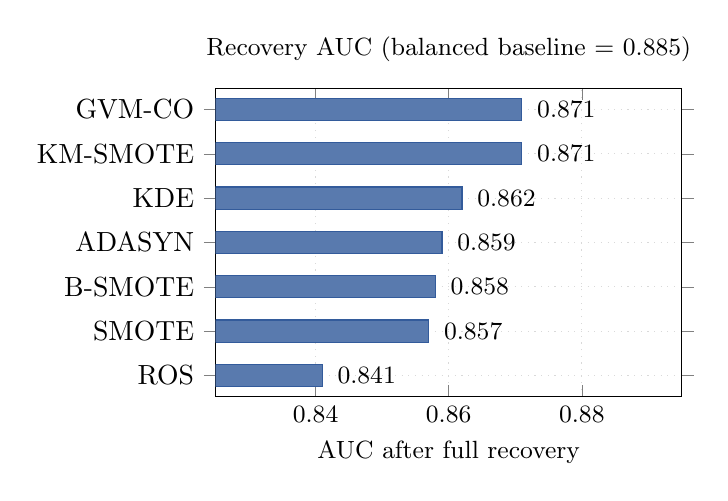
\begin{tikzpicture}
\begin{axis}[
  xbar,bar width=8pt,
  width=7.5cm,height=5.5cm,
  xlabel={\small AUC after full recovery},
  xmin=0.825,xmax=0.895,
  symbolic y coords={ROS,SMOTE,B-SMOTE,ADASYN,KDE,KM-SMOTE,GVM-CO},
  ytick=data,
  yticklabel style={font=\normalsize},
  xlabel style={font=\small},
  xticklabel style={font=\small},
  title={\small Recovery AUC (balanced baseline = 0.885)},
  title style={font=\small},
  nodes near coords,
  nodes near coords style={font=\small,xshift=2pt},
  every node near coord/.append style={/pgf/number format/.cd,fixed,precision=3},
  grid=major,grid style={dotted,gray!30},
  enlarge y limits=0.08]
\addplot[fill=myblue!65,draw=myblue!80] coordinates {
  (0.841,ROS)(0.857,SMOTE)(0.858,B-SMOTE)(0.859,ADASYN)
  (0.862,KDE)(0.871,KM-SMOTE)(0.871,GVM-CO)};
\end{axis}
\end{tikzpicture}

\column{0.46\textwidth}
\begin{center}
\begin{tabular}{@{}lcc@{}}
\toprule
Method & AUC & Gap \\
\midrule
Balanced baseline & 0.885 & --- \\
\midrule
GVM-CO     & 0.871 & $-0.014$ \\
KM-SMOTE   & 0.871 & $-0.014$ \\
KDE        & 0.862 & $-0.023$ \\
ADASYN     & 0.859 & $-0.026$ \\
B-SMOTE    & 0.858 & $-0.027$ \\
SMOTE      & 0.857 & $-0.028$ \\
ROS        & 0.841 & $-0.044$ \\
\bottomrule
\end{tabular}
\end{center}
\vspace{8pt}
\textbf{The 1.4\% residual gap is irreducible:}\\
Synthetic distributions cannot achieve $\NHOP=1$ against original minority when real minority is sparse.
By the TV identity: $\NHOP<1 \Rightarrow \TV>0 \Rightarrow$ information loss.

\textbf{Practical implication:} at high IR, prioritise data collection over algorithm choice.
\end{columns}
\end{frame}

% ----- Slide 5 ---------------------------------------------------------------
\begin{frame}{Causal Answer and Practical Implications}
\begin{columns}[T]
\column{0.50\textwidth}
\textbf{RQ6 (causality):} Yes — imbalance \emph{per se} degrades classifiers, independently of distributional shift or sample size reduction. Evidence: monotonic degradation with NHOP-shape preserved.

\vspace{8pt}
\textbf{RQ8 (recovery):} No oversampler achieves full recovery. Best ceiling: 98.4\% of balanced AUC (GVM-CO, KM-SMOTE). Gap explained by information-theoretic floor.

\column{0.48\textwidth}
\textbf{Practical implications:}
\begin{enumerate}
  \item At IR $< 2$: oversampling provides solid recovery (95--98\%)
  \item At IR $> 2$ (threshold zone): recovery degrades — invest in data collection
  \item LeakageSafeCV is a prerequisite — prevents 2--5\% AUC inflation that reverses rankings
  \item GVM-CO and KM-SMOTE are the recommended choices when oversampling is appropriate
\end{enumerate}
\end{columns}
\end{frame}

\end{document}
